\documentclass[11pt,a4paper]{article}
    \usepackage[margin=2.5cm]{geometry}
    \usepackage{enumitem}
    \usepackage{hyperref}
    \usepackage{tikz}
    \usetikzlibrary{arrows.meta,positioning,shapes.geometric}
    \title{Protein Structure Tools}
    \author{CBBL Tools}
    \date{\today}

    \tikzset{
      methodbox/.style={
        rounded corners=6pt,
        draw=blue!50!black,
        line width=0.9pt,
        fill=blue!6,
        minimum width=13cm,
        text width=11.8cm,
        align=left,
        inner sep=8pt
      }
    }

    \begin{document}
    \maketitle

    \section*{Scope}
    This folder groups utilities for downloading, splitting, aligning, and visualizing protein structures, mainly around PDB data, PyMOL, NGLView, and Bio.PDB.

    \section*{Material in this folder}
    \begin{itemize}[leftmargin=*]
\item \texttt{ChimeraAttempt.ipynb}
\item \texttt{IntroPymol.ipynb}
\item \texttt{frame\_observer.ipynb}
\item \texttt{align.py}
\item \texttt{chatmol.py}
\item \texttt{retrievePDB.py}
    \end{itemize}

    \section*{Method summary}
    \begin{itemize}[leftmargin=*]
\item \textbf{PDB retrieval and chain extraction}. The Bio.PDB-based script downloads structures and writes selected chains to separate coordinate files.
\item \textbf{Structural alignment in PyMOL}. The alignment script fetches structures and applies PyMOL alignment routines to compare folds or binding states.
\item \textbf{Interactive visualization}. The notebooks introduce PyMOL, Chimera-style workflows, and NGLView frame observation for structural inspection.
\item \textbf{LLM-assisted PyMOL commands}. The chatmol plugin stores conversation state and turns natural-language prompts into PyMOL commands through the OpenAI API.
    \end{itemize}

    \section*{Method scheme}
    Figure~\ref{fig:summary} is drawn directly in LaTeX with TikZ. It is a compact conceptual map of the main workflows discussed in this folder.

    \begin{figure}[ht]
    \centering
    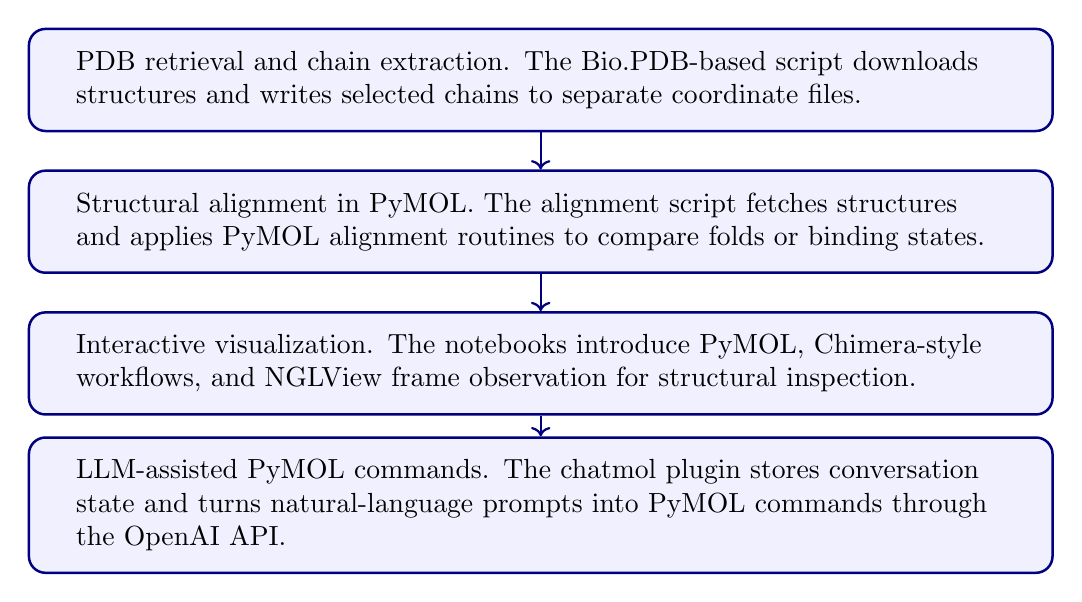
\begin{tikzpicture}[x=1cm,y=1cm]
    \node[methodbox] (m0) at (0,0.0) {PDB retrieval and chain extraction. The Bio.PDB-based script downloads structures and writes selected chains to separate coordinate files.};
    \node[methodbox] (m1) at (0,-1.8) {Structural alignment in PyMOL. The alignment script fetches structures and applies PyMOL alignment routines to compare folds or binding states.};
    \node[methodbox] (m2) at (0,-3.6) {Interactive visualization. The notebooks introduce PyMOL, Chimera-style workflows, and NGLView frame observation for structural inspection.};
    \node[methodbox] (m3) at (0,-5.4) {LLM-assisted PyMOL commands. The chatmol plugin stores conversation state and turns natural-language prompts into PyMOL commands through the OpenAI API.};
    \draw[->, thick, color=blue!50!black] (m0.south) -- (m1.north);
    \draw[->, thick, color=blue!50!black] (m1.south) -- (m2.north);
    \draw[->, thick, color=blue!50!black] (m2.south) -- (m3.north);
    \end{tikzpicture}
    \caption{Conceptual scheme for the methods in the PDBTools folder.}
    \label{fig:summary}
    \end{figure}

    \end{document}
